\documentclass[10pt,aspectratio=169]{beamer}
\usetheme[numbering=none,progressbar=none]{metropolis}

\usepackage[utf8]{inputenc}
\usepackage[T1]{fontenc}
\usepackage{lmodern}
\usepackage{microtype}
\usepackage{graphicx}
\usepackage[most]{tcolorbox}
\usepackage{xcolor}
\usepackage{tikz}
\usepackage{array}
\usepackage{ragged2e}
\usepackage{hyperref}
\usetikzlibrary{arrows.meta,calc,positioning}

% ---------- Palette ----------
\definecolor{bg}{HTML}{F5F8FD}
\definecolor{ink}{HTML}{0F1C33}
\definecolor{muted}{HTML}{64748B}
\definecolor{accent}{HTML}{255CFF}
\definecolor{accenttwo}{HTML}{0F9F7F}
\definecolor{sky}{HTML}{ECF3FF}
\definecolor{card}{HTML}{FFFFFF}
\definecolor{line}{HTML}{D9E4F2}
\definecolor{deep}{HTML}{12213F}
\definecolor{pillgreen}{HTML}{E7F7F0}
\definecolor{pillgold}{HTML}{FFF2DE}
\definecolor{gold}{HTML}{D39C39}

\hypersetup{colorlinks=true,urlcolor=accent}

% ---------- Beamer ----------
\setbeamersize{text margin left=7mm,text margin right=7mm}
\setbeamercolor{normal text}{fg=ink,bg=white}
\setbeamercolor{frametitle}{fg=ink,bg=white}
\setbeamercolor{framesubtitle}{fg=muted}
\setbeamercolor{title}{fg=ink}
\setbeamertemplate{navigation symbols}{}
\setbeamertemplate{headline}{}
\setbeamertemplate{footline}{}
\setbeamerfont{title}{size=\fontsize{30}{33}\selectfont,series=\bfseries}
\setbeamerfont{frametitle}{size=\fontsize{22}{24}\selectfont,series=\bfseries}
\setbeamerfont{framesubtitle}{size=\footnotesize}
\setbeamerfont{normal text}{size=\small}

\newcommand{\deckbackground}{%
\begin{tikzpicture}[remember picture,overlay]
\shade[left color=white,right color=bg] (current page.south west) rectangle (current page.north east);
\fill[accent!6] ([xshift=-0.7cm,yshift=-0.9cm]current page.north east) circle (2.6cm);
\fill[accenttwo!7] ([xshift=-1.0cm,yshift=0.8cm]current page.south east) circle (2.1cm);
\fill[accent!4] ([xshift=1.1cm,yshift=-0.5cm]current page.north west) circle (1.8cm);
\draw[line width=0.55pt,color=line] ([xshift=6mm,yshift=6mm]current page.south west) rectangle ([xshift=-6mm,yshift=-6mm]current page.north east);
\end{tikzpicture}%
}
\addtobeamertemplate{background canvas}{\deckbackground}{}

% ---------- Shared styles ----------
\tcbset{
  pitchcard/.style={
    enhanced,
    boxrule=0.65pt,
    colframe=line,
    colback=card,
    arc=5mm,
    left=2.5mm,
    right=2.5mm,
    top=2.5mm,
    bottom=2.5mm,
    before upper=\RaggedRight
  },
  darkcard/.style={
    enhanced,
    boxrule=0pt,
    colback=deep,
    coltext=white,
    arc=6mm,
    left=3.2mm,
    right=3.2mm,
    top=3.2mm,
    bottom=3.2mm,
    before upper=\RaggedRight
  }
}

% ---------- Helpers ----------
\newcommand{\eyebrow}[1]{%
\tcbox[on line,enhanced,boxrule=0pt,colback=sky,arc=4mm,left=2.2mm,right=2.2mm,top=1mm,bottom=1mm]{\footnotesize\bfseries\textcolor{accent}{\MakeUppercase{#1}}}%
}

\newcommand{\pill}[2]{%
\tcbox[on line,enhanced,boxrule=0pt,colback=#1,arc=6mm,left=2.6mm,right=2.6mm,top=1.1mm,bottom=1.1mm]{\scriptsize\bfseries #2}%
}

\newcommand{\infocard}[2]{%
\begin{tcolorbox}[pitchcard]
{\normalsize\bfseries #1}\\[0.8mm]
{\footnotesize\color{muted} #2}
\end{tcolorbox}
}

\newcommand{\stepcard}[3]{%
\begin{tcolorbox}[pitchcard]
{\footnotesize\bfseries\color{accent} #1}\\[0.8mm]
{\normalsize\bfseries #2}\\[0.8mm]
{\footnotesize\color{muted} #3}
\end{tcolorbox}
}

\newcommand{\thesisbox}[2]{%
\begin{tcolorbox}[darkcard]
{\footnotesize\bfseries\textcolor{white!68}{#1}}\\[1.5mm]
{\large\bfseries #2}
\end{tcolorbox}
}

\newcommand{\mockpanel}[3]{%
\begin{tcolorbox}[pitchcard,left=1.8mm,right=1.8mm,top=1.8mm,bottom=2.4mm]
\IfFileExists{#1}{%
  \centering\includegraphics[width=\linewidth,height=4.05cm,keepaspectratio]{#1}
}{%
  \begin{tcolorbox}[enhanced,boxrule=0pt,colback=deep,arc=4.5mm,height=4.05cm,valign=center,left=2mm,right=2mm,top=2mm,bottom=2mm]
    \centering
    {\Large\bfseries\color{white} Product Visual}\\[1mm]
    {\footnotesize\color{white!72} Add screenshot: \texttt{#1}}
  \end{tcolorbox}
}%
\vspace{1.5mm}
{\normalsize\bfseries #2}\\[0.8mm]
{\footnotesize\color{muted} #3}
\end{tcolorbox}
}

\newcommand{\roadstep}[2]{%
\begin{tcolorbox}[pitchcard]
{\footnotesize\bfseries\color{accent} STEP #1}\\[0.8mm]
{\normalsize\bfseries #2}
\end{tcolorbox}
}

\title{Block Lease}
\subtitle{Trusted rental deposits for student housing}
\author{}
\date{}

\begin{document}

% ---------- Slide 1 ----------
\begin{frame}[plain,shrink=6]
\begin{tikzpicture}[remember picture,overlay]
\shade[left color=white,right color=bg] (current page.south west) rectangle (current page.north east);
\fill[deep] ([xshift=2.25cm]current page.south east) rectangle (current page.north east);
\fill[accent] ([xshift=-1.5cm,yshift=-0.8cm]current page.north east) circle (2.1cm);
\fill[accenttwo!80] ([xshift=-0.7cm,yshift=0.8cm]current page.south east) circle (1.6cm);
\draw[line width=0.55pt,color=line] ([xshift=6mm,yshift=6mm]current page.south west) rectangle ([xshift=-6mm,yshift=-6mm]current page.north east);
\end{tikzpicture}

\vspace{1mm}
\begin{columns}[T,totalwidth=\textwidth]
\column{0.56\textwidth}
\eyebrow{Block Lease}\\[4mm]
{\fontsize{28}{31}\selectfont\bfseries Trusted deposits for student housing.}\\[3mm]
{\large\color{muted} Neutral escrow for cross-border move-ins, subleases, remote bookings, and lease takeovers.}\\[5mm]

\pill{pillgreen}{Cross-border ready}\hspace{1.5mm}
\pill{sky}{Neutral escrow}\hspace{1.5mm}
\pill{pillgold}{Built for subleases}\\[5mm]

{\small\color{muted} Instead of wiring a deposit to a stranger, the renter funds an escrow agreement until release or refund conditions are clearly defined.}\\[6mm]

\begin{tcolorbox}[pitchcard]
{\normalsize\bfseries The wedge is intentionally narrow}\\[1mm]
{\footnotesize\color{muted} Block Lease does not need to replace the housing marketplace. It only needs to de-risk the moment when both sides decide whether to commit.}
\end{tcolorbox}

\column{0.40\textwidth}
\begin{tcolorbox}[darkcard]
{\footnotesize\bfseries\textcolor{white!68}{Trust layer}}\\[2mm]
{\large\bfseries The risky transfer becomes a structured flow.}\\[1.2mm]
{\footnotesize\color{white!74} Move one step of the deal into neutral escrow, then release or refund based on the agreement outcome.}\\[5mm]

\begin{center}
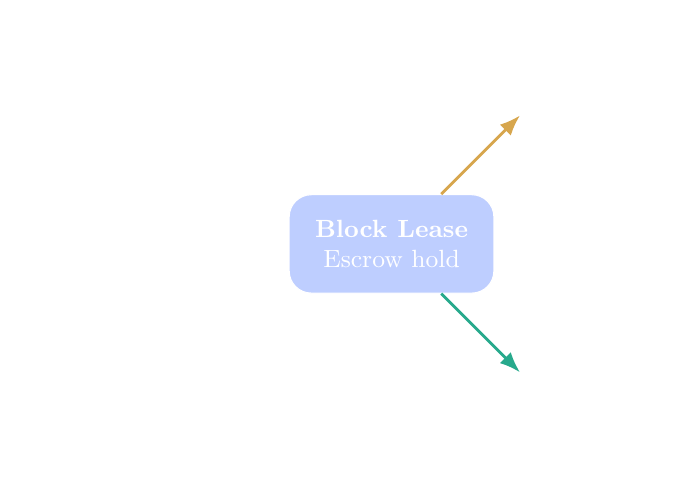
\begin{tikzpicture}[>=Latex,font=\small,node distance=7mm and 8mm]
\node[draw=white!18,fill=white!8,rounded corners=8pt,minimum width=2.5cm,minimum height=1.1cm,align=center,text=white] (renter) {\textbf{Renter}\\Funds deposit};
\node[draw=white!18,fill=accent!30,rounded corners=8pt,minimum width=2.6cm,minimum height=1.25cm,align=center,text=white,right=of renter] (escrow) {\textbf{Block Lease}\\Escrow hold};
\node[draw=white!18,fill=white!8,rounded corners=8pt,minimum width=2.55cm,minimum height=1.1cm,align=center,text=white,below right=10mm and -4mm of escrow] (payout) {\textbf{Release}\\Landlord};
\node[draw=white!18,fill=white!8,rounded corners=8pt,minimum width=2.55cm,minimum height=1.1cm,align=center,text=white,above right=10mm and -4mm of escrow] (refund) {\textbf{Refund}\\Renter};
\draw[->,line width=1pt,color=white] (renter) -- (escrow);
\draw[->,line width=1pt,color=accenttwo!90] (escrow) -- (payout);
\draw[->,line width=1pt,color=gold!90] (escrow) -- (refund);
\end{tikzpicture}
\end{center}

\vspace{4mm}
\begin{tcolorbox}[enhanced,boxrule=0pt,colback=white!8,arc=4mm,left=3mm,right=3mm,top=2.4mm,bottom=2.4mm]
{\footnotesize\color{white!88} A safer commitment path for both sides, without asking users to trust each other first.}
\end{tcolorbox}
\end{tcolorbox}
\end{columns}
\end{frame}

% ---------- Slide 2 ----------
\begin{frame}[shrink=5]{The Problem}
\begin{columns}[T,totalwidth=\textwidth]
\column{0.40\textwidth}
{\Large\bfseries The pain is not discovery. It is commitment.}\\[4mm]
{\footnotesize\color{muted} Student housing moves fast, across distance, and between people who often do not know each other well. The deposit becomes the most stressful and least reversible step. The market does not need another listing site. It needs a commitment layer.}\\[5mm]

\begin{tcolorbox}[darkcard]
{\footnotesize\bfseries\textcolor{white!68}{Core insight}}\\[2mm]
{\Large\bfseries Trust breaks before keys change hands.}
\end{tcolorbox}

\column{0.56\textwidth}
\infocard{For renters}{Sending a deposit directly to an unfamiliar person feels like the most irreversible step, especially before arrival or an in-person viewing.}
\vspace{1.8mm}
\infocard{For landlords and sublessors}{Holding a room for a remote or first-time renter feels risky without a credible commitment signal and a clear funding path.}
\end{columns}
\end{frame}

% ---------- Slide 3 ----------
\begin{frame}[shrink=6]{Where Block Lease Wins First}
\begin{columns}[T,totalwidth=\textwidth]
\column{0.54\textwidth}
\begin{columns}[T,totalwidth=\linewidth]
\column{0.49\linewidth}
\infocard{Cross-border move-ins}{Students may need to secure housing before they have local banking history, a U.S.\ account, or the ability to visit in person.}
\vspace{1.6mm}
\infocard{Remote booking}{A renter may commit from abroad or another city before seeing the room, making the deposit decision unusually exposed.}
\column{0.49\linewidth}
\infocard{Student-to-student subleases}{Semester and summer subleases often happen between peers who have never met, even though the room and timing are real.}
\vspace{1.6mm}
\infocard{Lease takeovers}{When one student replaces another mid-lease, a clear deposit path reduces confusion during a rushed handoff.}
\end{columns}

\column{0.42\textwidth}
\thesisbox{Why this matters}{The same product wedge solves several situations where housing demand is real, urgency is high, and direct payment feels unsafe.}
\vspace{2.4mm}
\begin{tcolorbox}[pitchcard]
{\normalsize\bfseries Strategic advantage}\\[1mm]
{\footnotesize\color{muted} Block Lease can work alongside campus communities, student housing operators, and international student channels instead of competing with them for listings.}
\end{tcolorbox}
\end{columns}
\end{frame}

% ---------- Slide 4 ----------
\begin{frame}[shrink=5]{How It Works}
\begin{columns}[T,totalwidth=\textwidth]
\column{0.55\textwidth}
\begin{tcolorbox}[pitchcard,left=4mm,right=4mm,top=4mm,bottom=4mm]
{\normalsize\bfseries Escrow flow}\\[4mm]
\begin{center}
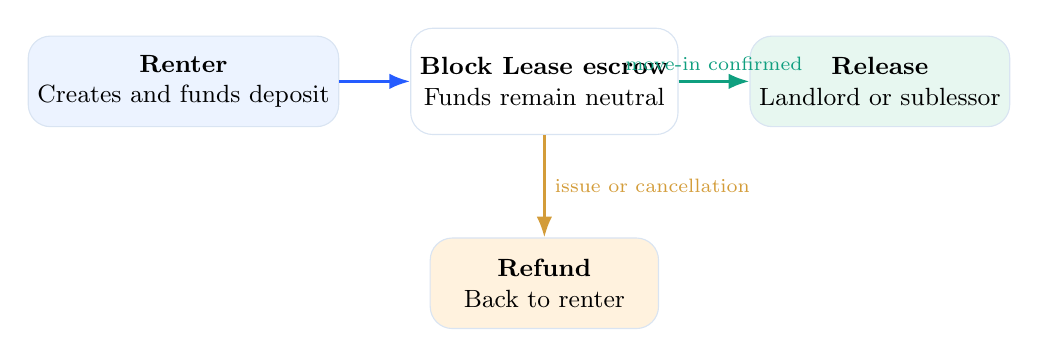
\begin{tikzpicture}[>=Latex,font=\small,node distance=8mm and 9mm]
\node[draw=line,fill=sky,rounded corners=8pt,minimum width=3.05cm,minimum height=1.15cm,align=center] (renter) {\textbf{Renter}\\Creates and funds deposit};
\node[draw=line,fill=card,rounded corners=8pt,minimum width=3.25cm,minimum height=1.35cm,align=center,right=of renter] (escrow) {\textbf{Block Lease escrow}\\Funds remain neutral};
\node[draw=line,fill=pillgreen,rounded corners=8pt,minimum width=2.9cm,minimum height=1.15cm,align=center,right=of escrow] (release) {\textbf{Release}\\Landlord or sublessor};
\node[draw=line,fill=pillgold,rounded corners=8pt,minimum width=2.9cm,minimum height=1.15cm,align=center,below=13mm of escrow] (refund) {\textbf{Refund}\\Back to renter};
\draw[->,line width=1pt,color=accent] (renter) -- (escrow);
\draw[->,line width=1pt,color=accenttwo] (escrow) -- node[above,midway,font=\scriptsize\color{muted}]{move-in confirmed} (release);
\draw[->,line width=1pt,color=gold] (escrow) -- node[right,font=\scriptsize\color{muted}]{issue or cancellation} (refund);
\end{tikzpicture}
\end{center}
\vspace{2mm}
{\footnotesize\color{muted} Funds stay neutral until the agreement reaches a clear outcome.}
\end{tcolorbox}

\column{0.41\textwidth}
\stepcard{01}{Create agreement}{Set the parties, property, deposit amount, and release conditions.}
\vspace{1.8mm}
\stepcard{02}{Hold the deposit}{Keep funds in escrow instead of sending them directly to the other side too early.}
\vspace{1.8mm}
\begin{tcolorbox}[pitchcard,colback=sky,colframe=sky]
{\footnotesize\bfseries\color{accent} 03}\\[0.8mm]
{\normalsize\bfseries Resolve the outcome}\\[0.8mm]
{\footnotesize\color{ink} Release, refund, or review based on the agreement state.}
\end{tcolorbox}
\end{columns}
\end{frame}

% ---------- Slide 5 ----------
\begin{frame}[shrink=4]{Prototype Today}
\begin{columns}[T,totalwidth=\textwidth]
\column{0.49\textwidth}
\mockpanel{4ec44838-7908-4030-a02c-d6b510981f8c.png}{Escrow dashboard}{Track active agreements, statuses, deposits, and next actions from one operations view.}

\column{0.49\textwidth}
\mockpanel{725e710f-4d4e-4077-8392-7fbfa4a03693.png}{Agreement workspace}{Open a single agreement to review parties, property, deposit amount, timeline, and payout status.}
\end{columns}
\end{frame}

% ---------- Slide 6 ----------
\begin{frame}[shrink=6]{Business Model}
\begin{columns}[T,totalwidth=\textwidth]
\column{0.39\textwidth}
\thesisbox{Why users pay}{Block Lease reduces deposit risk for renters while increasing payment confidence for landlords and sublessors.}
\vspace{2mm}
\begin{tcolorbox}[pitchcard]
{\normalsize\bfseries Go-to-market shape}\\[1mm]
{\footnotesize\color{muted} Start where trust friction is already obvious: student housing operators, sublease communities, and international student channels.}
\end{tcolorbox}
\vspace{2mm}
\begin{tcolorbox}[pitchcard,colback=sky,colframe=sky]
{\normalsize\bfseries Defensible wedge}\\[1mm]
{\footnotesize\color{ink} The fee is attached to a high-stress transaction moment where both sides benefit from structure.}
\end{tcolorbox}

\column{0.57\textwidth}
\begin{columns}[T,totalwidth=\linewidth]
\column{0.49\linewidth}
\infocard{Transaction fee}{Charge a small fee per escrow agreement once funds are placed into the protected flow.}
\vspace{1.6mm}
\infocard{Verification services}{Offer school email checks, identity verification, and renter or landlord trust signals as premium services.}
\column{0.49\linewidth}
\infocard{Partner distribution}{Work with student housing operators, campus communities, and international student programs that already source demand.}
\vspace{1.6mm}
\infocard{Expansion path}{Add dispute handling, payout tooling, and reputation signals as the product matures.}
\end{columns}
\end{columns}
\end{frame}

% ---------- Slide 7 ----------
\begin{frame}[shrink=8]{Infrastructure Roadmap}
\begin{columns}[T,totalwidth=\textwidth]
\column{0.40\textwidth}
\infocard{Why smart contracts later}{Escrow is fundamentally a conditional transfer problem, which makes rule-based automation a natural long-term fit.}
\vspace{1.8mm}
\infocard{Why stablecoins}{Deposits should preserve value and settle predictably, which makes a dollar-backed asset more usable than a volatile token.}

\column{0.56\textwidth}
\begin{tcolorbox}[pitchcard,left=4mm,right=4mm,top=4mm,bottom=4mm]
{\Large\bfseries Suggested roadmap}\\[4mm]
\textcolor{accent}{\bfseries 1}\hspace{2mm}{\small Launch the escrow workflow and prove the user story.}\\[2mm]
\textcolor{accent}{\bfseries 2}\hspace{2mm}{\small Standardize agreement states, release rules, and review operations.}\\[2mm]
\textcolor{accent}{\bfseries 3}\hspace{2mm}{\small Add stablecoin settlement on an EVM Layer 2 such as Base.}\\[2mm]
\textcolor{accent}{\bfseries 4}\hspace{2mm}{\small Expand into dispute automation, partner tooling, and policy controls.}
\vspace{2mm}
{\footnotesize\color{muted} Use an EVM Layer 2 when it improves fees, speed, and consumer UX.}
\end{tcolorbox}
\end{columns}
\end{frame}

% ---------- Slide 8 ----------
\begin{frame}[plain]
\begin{center}
\begin{tcolorbox}[darkcard,width=0.92\linewidth,left=7mm,right=7mm,top=6mm,bottom=6mm]
\centering
{\footnotesize\bfseries\textcolor{white!68}{BLOCK LEASE}}\\[4mm]
{\fontsize{22}{25}\selectfont\bfseries\color{white} The trust layer for the most fragile dollar in student housing.}\\[3mm]
{\normalsize\color{white!80} A safer commitment path for cross-border move-ins, subleases, and remote rentals.}\\[6mm]

\begin{tcolorbox}[enhanced,boxrule=0pt,colback=white,arc=7mm,left=8mm,right=8mm,top=5mm,bottom=5mm,width=0.78\linewidth]
\centering
{\Large\bfseries One-line pitch}\\[2.5mm]
{\normalsize Instead of asking a student to send a deposit directly to a stranger, Block Lease puts the money into escrow until the outcome is clear.}
\end{tcolorbox}

\end{tcolorbox}
\end{center}
\end{frame}

\end{document}
